\section{Wykorzystane wzorce projektowe}
\subsection{Strategia}
Wzorzec projektowy strategia to behawioralny wzorzec projektowy, który umożliwia definiowanie rodziny algorytmów, enkapsulowanie każdego z nich oraz uczynienie ich wymienialnymi. Wzorzec ten pozwala na zmienianie algorytmów niezależnie od klientów, które z nich korzystają. Główne elementy wzorca Strategia to: Kontekst (Context), Strategia (Strategy) oraz Konkretne Strategie (Concrete Strategies). Kontekst to klasa, która zawiera referencję do obiektu Strategii i deleguje do niego wykonanie pewnych operacji. Strategia to interfejs wspólny dla wszystkich algorytmów, który definiuje metodę, jaką muszą implementować wszystkie konkretne strategie. Konkretne Strategie to klasy implementujące interfejs Strategii, zawierające konkretne algorytmy. Wzorzec Strategia jest użyteczny, gdy istnieje potrzeba dynamicznego wyboru algorytmu w trakcie działania programu lub gdy chcemy uniknąć umieszczania wielu złożonych warunków w kodzie. Dzięki temu wzorcowi kod staje się bardziej elastyczny i łatwiejszy do utrzymania.

W przypadku naszego projektu, użyliśmy tego wzorca do implementacji dostawców formatów (konwerterów)
\begin{figure}[ht]
	\centering
	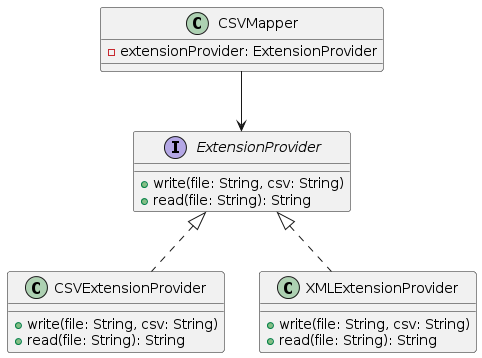
\includegraphics[width=0.65\textwidth]{materiały/strategia}
	\caption{Wykorzystanie strategii}
\end{figure}

\subsection{Iterator}
Iterator to behawioralny wzorzec projektowy, który umożliwia sekwencyjne przechodzenie przez elementy kolekcji bez ujawniania jej wewnętrznej struktury (takiej jak lista, stos, drzewo, itp.). Dzięki temu wzorcowi można uzyskać jednolity interfejs do przeglądania różnych typów kolekcji, co ułatwia manipulację i przetwarzanie danych. Główne elementy wzorca Iterator to: Iterator, Kolekcja (Collection) oraz Konkretne Iteratory (Concrete Iterators). Iterator to interfejs definiujący metody do iterowania po elementach kolekcji, takie jak hasNext() (sprawdzająca, czy są jeszcze elementy do przejścia) oraz next() (zwracająca kolejny element). Konkretne Iteratory to klasy implementujące interfejs Iteratora, które zawierają logikę potrzebną do przechodzenia po konkretnej strukturze danych.

\paragraph{} W przypadku naszego projektu, użyliśmy tego wzorca do implementacji wykrywania adnotacji w klasach wykorzystujących mappera.

\begin{figure}[ht]
	\centering
	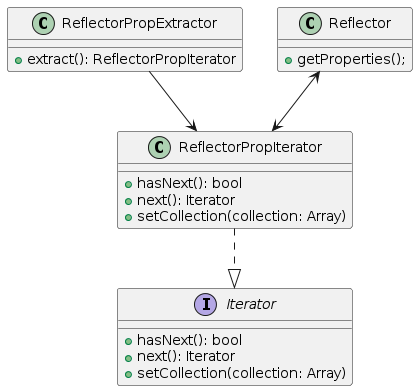
\includegraphics[width=0.6\textwidth]{materiały/iterator}
	\caption{Wykorzystanie iteratora}
\end{figure}

\subsection{Łańcuch zobowiązań}
Łańcuch zobowiązań to behawioralny wzorzec projektowy, który pozwala przekazywać żądania wzdłuż łańcucha obiektów obsługujących. Otrzymawszy żądanie, każdy z obiektów obsługujących decyduje o jego przetworzeniu lub przekazaniu do kolejnego obiektu obsługującego w łańcuchu. Wzorzec ten jest użyteczny, gdy chcemy oddzielić nadawcę żądania od jego odbiorcy oraz zapewnić możliwość dynamicznego konfigurowania łańcucha obiektów obsługujących. Dzięki temu wzorcowi możemy łatwo modyfikować kolejność i liczbę obiektów przetwarzających żądanie, co zwiększa elastyczność i łatwość utrzymania kodu.

\paragraph{} W przypadku naszego projektu, użyliśmy tego wzorca prawie w całym projekcie. Kod był pisany w taki sposób aby można było go rozwijać na każdym etapie, dzięki czemu naturalnie wyłoniła się struktura łańcucha.

\begin{figure}[ht]
	\centering
	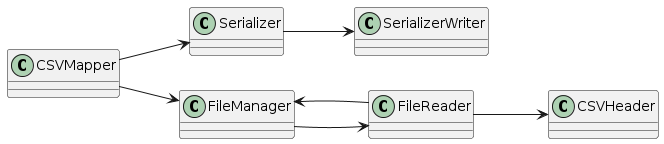
\includegraphics[width=1.0\textwidth]{materiały/lancuch}
	\caption{Wykorzystanie łańcucha zobowiązań}
\end{figure}

\subsection{Dekoratror}
Dekorator to strukturalny wzorzec projektowy, który pozwala dynamicznie dodawać nowe obowiązki obiektom poprzez umieszczanie tych obiektów w specjalnych obiektach opakowujących, które zawierają odpowiednie zachowania. Dzięki temu wzorcowi można rozszerzać funkcjonalność obiektów bez modyfikowania ich kodu bazowego. W kontekście PHP, dekorator może być również implementowany za pomocą cech (traits). Traits w PHP to mechanizm pozwalający na wielokrotne wykorzystanie kodu w różnych klasach.

\begin{figure}[ht]
	\centering
	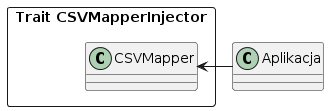
\includegraphics[width=0.4\textwidth]{materiały/dekorator}
	\caption{Wykorzystanie dekoratora}
\end{figure} 